\documentclass[12pt]{article}
\usepackage[spanish]{babel}
\usepackage{graphicx}
\usepackage{amsmath}
\usepackage[margin=2.5cm]{geometry}
\usepackage{amssymb}
\usepackage{float}
\usepackage{caption}

\title{Difusión de calor}
\author{Brayan Matias Rojo}
\date{June 2025}

\renewcommand{\baselinestretch}{1.5}

\begin{document}

\tableofcontents

\newpage

\section{Introducción}

El concepto de calor ha acompañado a la humanidad desde la antigüedad siendo utilizado para describir lo caliente o frio se siente un objeto tomando en cuenta nuestro sentido del tacto (idea que aun hoy en día persiste en el lenguaje coloquial). Serían los griegos como Aristóteles o Heráclito quienes darían las primeras descripciones sobre el calor, considerando que se trataba de un estado en el que se podría encontrar a la materia o una cualidad. \\

En el siglo XVII se tenía la idea de que existía un fluido calórico compuesto de pequeñas partículas, que al transmitirse de un cuerpo a otro podían alterar la temperatura de estos. De esta manera si dos objetos se ponían en contacto, dicha sustancia se movería del cuerpo más caliente al más frío. Posteriormente, los trabajos experimentales de James Joule y Julius von Mayer en 1811 y 1842 mostrarían la relación existente entre el calor y el trabajo mecánico, llegando así a la idea de que el calor no es más que otra forma de energía. \\

Sería en esta época donde Joseph Fourier realizaría su trabajo con el objetivo de dar una descripción de cómo el calor se distribuye a lo largo de una región, llegando así a la ecuación del calor y al desarrollo de las series de Fourier. A finales del siglo XIX fue cuando Maxwell, Boltzmann y Bernoulli llegarían a la Teoría Cinética de los Gases dando forma al concepto moderno de calor como la energía que se transfiere de un sistema termodinámico a otro debido a la diferencia de sus temperaturas. \\

De esta manera, la idea de calor ha tenido muchos cambios a lo largo de la historia hasta tomar la forma que hoy en día es físicamente aceptada, dándonos en el proceso un mejor entendimiento sobre la materia y su composición. En la actualidad la investigación sobre el calor sigue teniendo una gran relevancia en los campos de la ingeniería, la física, etc, siendo de especial interés el saber cómo es que dicha forma de energía se transmite y distribuye en distintos objetos y materiales. \\

\subsection{Marco Teórico}
\subsubsection{Conceptos iniciales}

Los átomos y/o moléculas que componen a un objeto están en constante movimiento, por lo que tienen una velocidad asociada y, por ende, una energía cinética. Podemos entender la \textbf{temperatura} de un objeto como una medida de la energía cinética que en promedio tienen las partículas que conforman a dicho cuerpo. \\

Si ahora suponemos que tenemos dos objetos con diferentes temperaturas y los ponemos en contacto, las partículas que los componen, en promedio se mueven a diferentes velocidades lo que hace más probable que los átomos y/o moléculas del cuerpo con mayor temperatura le transfieran energía a las partículas del cuerpo con menor temperatura debido a las colisiones entre estas. De esta forma, hay una transferencia de energía neta del cuerpo con mayor temperatura al cuerpo con menor temperatura. A este proceso en el que se transfiere energía entre dos sistemas en contacto debido a la diferencia de temperaturas es lo que conocemos como \textbf{calor}. Existen tres formas en las que se puede dar la transferencia de calor: conducción, convección y radiación. En este trabajo serán de especial interés las dos primeras. \\ 

Para ejemplificar el proceso de transferencia de calor por \textbf{conducción}, consideremos un gas en el cual hay un gradiente de temperatura. Debido a esto hay zonas donde las partículas tienen una mayor energía cinética en promedio que en otras partes del mismo gas. Si no hay un movimiento global en las partículas, la única forma en la que habrá transferencia de energía será debido a las colisiones entre partículas vecinas, lo que hace que la energía se mueva a aquellos puntos en los que la temperatura es menor. Así, la transferencia de calor por conducción se debe al movimiento microscópico de los átomos/moléculas que conforman a un cuerpo. En líquidos y sólidos el proceso es análogo, sin embargo las fuerzas que unen a las partículas son más grandes y están menos espaciadas por lo que los efectos pueden diferir. \\

Por otro lado, cuando hay un movimiento macroscópico de un fluido frente a una diferencia de temperaturas, entonces tenemos transferencia de calor por \textbf{convección}. Es importante resaltar que si la velocidad de un fluido es cero (esta en reposo) entonces no puede haber convección. Podemos tener una convección forzada cuando el movimiento del fluido se debe a factores externos como en un sistema de ventilación, o podemos tener una convección libre cuando el fluido se desplaza debido a fuerzas de empuje por diferencias de densidad, como cuando el agua hirviendo en una olla se transforma en vapor de agua y este asciende, transmitiendo así calor con sus alrededores. \\

De esta manera, tenemos un concepto claro de temperatura y calor, así como de dos de los procesos en los que la energía térmica se puede transferir de un sistema a otro. Ahora necesitamos un modelo matemático para describir cómo es que se da dicha transferencia a lo largo del tiempo y el espacio. \\

\subsubsection{Desarrollo de la ecuación de calor (1 Dimensión)}

Para encontrar una ecuación que pueda modelar la transferencia de calor iniciaremos en el caso de una dimensión, es decir, supondremos que el calor se transmite en una única dirección. Para esto consideremos una barra conductora de calor en la cual hay un gradiente de temperatura. Para que se cumpla la condición de que el calor fluya en una sola dirección, tomaremos en cuenta que la superficie lateral de la barra esta completamente aislada. Además de esto, para simplificar el desarrollo de la expresión que buscamos, se supondrá que la barra tiene una densidad uniforme así como un calor especifico constante (lo cual es una buena aproximación en algunos intervalos de temperatura según el material que se maneje). \\

\begin{figure}[H]
\begin{center}
    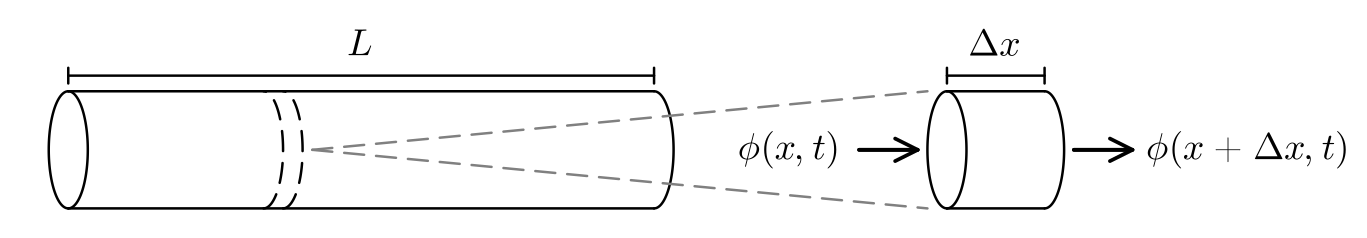
\includegraphics[width=1\linewidth]{Barra.png}
    \caption{Diagrama del flujo de calor en un elemento diferencial de una barra conductora de calor.}
\end{center}
\end{figure}

\newpage

Definimos $\phi$ como el flujo de energía térmica, es decir, la energía en forma de calor que fluye por la barra por unidad de tiempo y por unidad de área. Este flujo depende tanto de la posición de la barra como del tiempo en el que se mida, por lo que $\phi(x,t)$ es una función tanto del espacio (en este caso en la dirección $x$) como del tiempo. Si tomamos en cuenta una sección transversal de la barra con grosor $\Delta x$ podemos ver que, por conservación de la energía, el cambio en la calor en el punto $x$ depende de cuánta energía entra y cuánta energía sale, lo que nos lleva a la expresión:

\begin{align}
    \frac{\partial Q}{\partial t}\Big|_x  \approx A\cdot\phi(x,t) - A\cdot\phi(x+\Delta x,t)
\end{align}

donde $Q$ es el calor, mientras que $A$ es el área transversal del tubo. Hay que mencionar que también es posible que se genere calor dentro de la sección de grosor $\Delta x$ debido a a una reacción química, una corriente eléctrica o algún otro fenómeno, por lo que se debería agregar un termino correspondiente a dicha contribución en la ecuación (1), sin embargo para nuestro modelo supondremos que la única forma en la que puede pasar calor a través de la sección transversal es debido al flujo $\phi(x,t)$. \\

Ahora nos interesa que la ecuación (1) quede en términos de la temperatura, pues es una magnitud física que resulta más fácil de medir y estudiar que el calor. Para esto consideraremos la ecuación de calor especifico, que nos dice que el calor que entra o sale de un sistema $\Delta Q$ es directamente proporcional a la masa de dicho sistema y al cambio en su temperatura $\Delta T$. La constante de proporcionalidad que relaciona estas cantidades es el calor especifico $c$ que es la cantidad de energía necesaria para aumentar la temperatura de una unidad de masa en una unidad de temperatura.

\begin{align}
    \Delta Q = mc\Delta T
\end{align}

Específicamente queremos saber cómo es la tasa de cambio del calor, por lo que tomaremos en cuenta un intervalo de tiempo $\Delta t$ en el que se de la transferencia de calor. Además de esto, si utilizamos la relación entre masa y densidad $\rho = m/V$, tenemos el siguiente desarrollo:

\begin{align*}
    \Delta Q = \rho cV\Delta T \;\;\;\; \Rightarrow \;\;\;\; \Delta Q = \rho cA\Delta x\Delta T \;\;\;\; \Rightarrow \;\;\;\; \frac{\Delta Q}{\Delta t} = \rho cA\Delta x\frac{\Delta T}{\Delta t}
\end{align*}

tomando el limite cuando $\Delta t \rightarrow 0$ llegamos a la expresión:

\begin{align}
    \frac{\partial Q}{\partial t} = \rho cA\Delta x\frac{\partial T}{\partial t}
\end{align}

sustituyendo esta expresión en la ecuación (1) tenemos lo siguiente:

\begin{align}
    \rho c\Delta x\frac{\partial T}{\partial t}\Big|_x  \approx \phi(x,t) - \phi(x+\Delta x,t)
\end{align}

Esta se trata de una aproximación puesto que estamos considerando un grosor $\Delta x$ para calcular el cambio de la energía en el punto $x$, sin embargo esta aproximación mejora si reducimos el tamaño de dicho grosor, es decir, si tomamos el limite cuando $\Delta x \rightarrow 0$. Si reordenamos los términos de la ecuación (4) y tomamos el limite tenemos entonces que:

\begin{align}
    \nonumber \rho c\frac{\partial T}{\partial t}\Big|_x  = \lim_{\Delta x \to 0} \frac{\phi(x,t) - \phi(x+\Delta x,t)}{\Delta x}& = -\lim_{\Delta x \to 0} \frac{\phi(x+\Delta x,t)-\phi(x,t)}{\Delta x} \\
    \nonumber \\
    \Rightarrow \;\;\rho c\frac{\partial T}{\partial t} = &-\frac{\partial \phi}{\partial x}
\end{align}

Esta expresión nos da una ecuación con dos variables, por lo que si queremos simplificarla, debemos encontrar una relación entre el flujo de energía térmica y la temperatura, lo cual parece tener sentido si recordamos que la transmisión de calor se da justamente por una diferencia de temperaturas. La relación que buscamos entre estas dos variables debe cumplir con las siguientes consideraciones: \\

\begin{enumerate}
    \item Si no hay una diferencia o gradiente de temperaturas, entonces no hay flujo de calor.
    \item Cuando hay una diferencia de temperaturas, el flujo de calor debe ir de la zona con mayor temperatura a la zona con menor temperatura.
    \item Entre menor sea la diferencia de temperaturas, menor será el flujo de calor.
    \item La cantidad de calor que fluye depende del material en el que se de dicha transmisión de energía.
\end{enumerate}

El modelo que mejor se ajusta a estas condiciones es la \textbf{Ley de Fourier} dada por la expresión:

\begin{align}
    \phi = -K_0\frac{\partial T}{\partial x}
\end{align}

donde $K_0$ es una constante del material en el que se da el flujo de calor y que se conoce como \textbf{conductividad térmica}. De esta manera $K_0$ es una medida de qué tan buen conductor de calor es un objeto. si sustituimos esta ecuación en (5) tenemos lo siguiente:

\begin{align*}
    \rho c\frac{\partial T}{\partial t} = \frac{\partial }{\partial x}\left( K_0\frac{\partial T}{\partial x} \right)
\end{align*}

Es importante mencionar que la conductividad térmica puede cambiar si la temperatura del material cambia, sin embargo si el intervalo en el que varia la temperatura no es muy grande, podemos aproximar a $K_0$ como una constante, de tal manera que puede salir de la derivada sin problemas. Así llegamos a la ecuación de calor que buscamos:

\begin{align}
    \frac{\partial T}{\partial t} = \kappa\frac{\partial^2 T}{\partial x^2}
\end{align}

donde $\kappa = K_0/\rho c$ la conocemos como \textbf{difusividad térmica}. Al igual que con $K_0$, la difusividad térmica no es una constante pues varía dependiendo de la temperatura a la que se encuentre el material, sin embargo, como ya se mencionó si consideramos un intervalo de temperatura no muy grande, es posible aproximar esta propiedad a una constante. \\

\subsubsection{Desarrollo de la ecuación de calor (2 o 3 Dimensiones)}

Con el desarrollo de la sección anterior obtuvimos una expresión para describir cómo es el cambio en la temperatura de un sistema cuando el flujo de calor solo se da en una dirección. Para hacer el mismo análisis, esta vez considerando dos o tres dimensiones, es necesario definir la variable $\epsilon (\vec{r})$ como la densidad de energía térmica y considerar una región cerrada $R$. De esta manera, la cantidad de energía térmica contenida en dicha región es:

\begin{align*}
    Q = \int_R \epsilon(\vec{r})dV
\end{align*}

si modificamos la ecuación (2) de calor especifico tenemos:

\begin{align*}
    \epsilon(\vec{r}) = \rho cT \;\;\;\; \Rightarrow \;\;\;\; Q = \int_R \rho cT(\vec{r}) \; dV
\end{align*}

Por otro lado, es necesario un vector que nos indique la cantidad de energía térmica que esta entrando o saliendo de la región $R$ y en qué dirección lo esta haciendo. De esta manera tenemos $\vec{\phi}(\vec{r},t)$ como el vector de flujo de calor. Es importante señalar que, si la dirección de este vector es paralela a la frontera en algún punto, entonces no hay flujo de calor hacia el exterior o el interior. Por ello necesitamos considerar solo la componente normal a la frontera de $\vec{\phi}(\vec{r},t)$. Si integramos esta cantidad a lo largo de toda la frontera de $R$ tenemos entonces el cambio en la energía térmica de dicha región de la siguiente manera:

\begin{align*}
    \frac{d}{dt}\int_R \rho cT(\vec{r}) \; dV = - \oint_{\partial R} \vec{\phi}(\vec{r},t)\cdot \hat{n} \; dS 
\end{align*}

El signo negativo nos indica que cuando hay una salida del flujo de calor, entonces hay una disminución en la energía térmica de la región $R$. Al igual que en el caso unidimensional, consideramos que no hay generación de energía dentro de la región $R$. Si ahora aplicamos el teorema de Gauss a la integral del vector $\vec{\phi}(\vec{r},t)$ e intercambiamos la derivada por la integral del lado izquierdo de la expresión (lo cual es valido pues consideramos que $R$ no cambia con el tiempo y que la función de temperatura es continua) tenemos entonces:

\begin{align*}
    \int_R \rho c\frac{\partial T}{\partial t} \; dV = - \int_{R} \nabla \cdot\vec{\phi}\; dV \;\;\;\; \Rightarrow \;\;\;\; \int_R \left[\rho c\frac{\partial T}{\partial t} + \nabla \cdot\vec{\phi}\right]\; dV = 0
\end{align*}

como esta integral debe ser cero para cualquier región cerrada $R$, se deduce entonces que la función dentro de la integral es exactamente cero, así llegamos entonces a la expresión:

\begin{align}
    \rho c\frac{\partial T}{\partial t} = - \nabla \cdot\vec{\phi}
\end{align}

\begin{figure}[H]
\begin{center}
    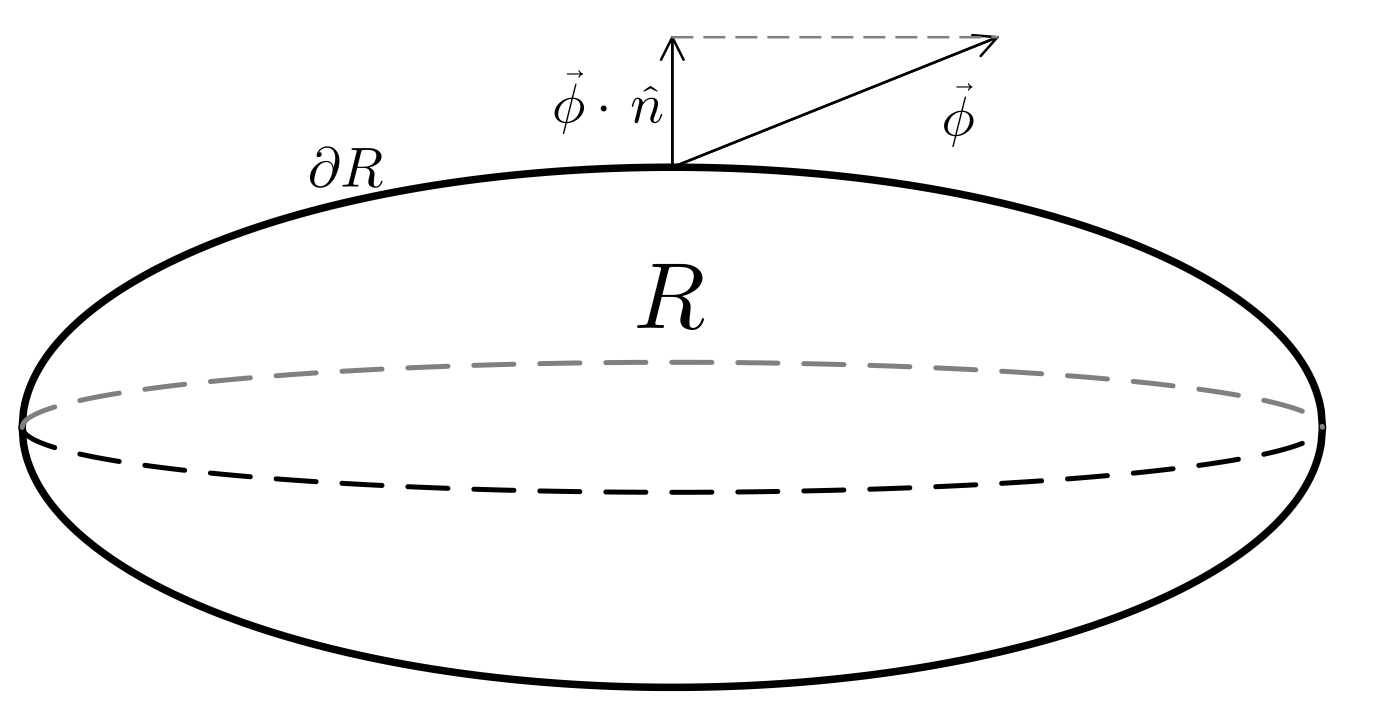
\includegraphics[width=0.8\linewidth]{Region_R.png}
    \caption{Componente normal del flujo de calor en una región cerrada.}
\end{center}
\end{figure}

Si queremos simplificar aún más esta expresión es necesario utilizar la ley de Fourier para el caso tridimensional, dada por la ecuación:

\begin{align}
    \vec{\phi} = -K_0\nabla T
\end{align}

donde se sustituye a la parcial con respecto del tiempo por el gradiente, lo que asegura que el flujo de calor se de en la dirección opuesta a donde la temperatura tiene un mayor aumento. Si sustituimos esta expresión en la ecuación (8) obtenemos entonces:

\begin{align}
    \frac{\partial T}{\partial t} = \kappa \nabla^2 T
\end{align}

donde $\nabla^2$ es el operador Laplaciano y $\kappa$ es la misma difusividad térmica definida para el caso unidimensional.

\subsubsection{Ecuaciones diferenciales parciales}

Como podemos ver, las expresiones (7) y (10) se tratan de ecuaciones diferenciales parciales de segundo orden para la temperatura. Este tipo de ecuaciones nos sirven para modelar cómo es que cambia la función involucrada con respecto de ciertas variables (en este caso el tiempo y el espacio). En este caso, ambas ecuaciones señalan que la derivada de la temperatura con respeto del tiempo es proporcional a la segunda deriva de la temperatura con respecto del espacio de la misma temperatura. Esto cobra sentido si consideramos que la segunda derivada de una función nos habla de la curvatura de la misma. Por otro lado, en una gráfica de temperatura vs posición podemos ver que la curvatura nos indica una diferencia de temperatura en un punto con respecto a sus alrededores, por lo que el cambio de la temperatura con respecto al tiempo será mayor en aquellos puntos donde esta curvatura sea más pronunciada debido al intercambio de energía en forma de calor. \\

A pesar de que estas ecuaciones son útiles para modelar el comportamiento de la función de temperatura, no es posible encontrar la solución a esta solo con dichas ecuaciones. Para encontrar la solución y así conocer la distribución de temperatura para cualquier instante en el tiempo a lo largo de un intervalo en el caso de una dimensión, o en todo una región en el caso bidimensional y tridimensional, necesitamos dos condiciones: una condición inicial y una condición de frontera. La primera se trata de conocer cómo es la distribución de la temperatura en el instante inicial ($t=0$):

\begin{align*}
    & T(x,0) = f(x) \;\;\;\;\;\;\;\; (\text{1 dimensión}) \\
    &T(\vec{r},0) = f(\vec{r}) \;\;\;\;\;\;\;\; (\text{2 o 3 dimensiones})
\end{align*}

Para la segunda condición, debemos proporcionar información del comportamiento de la temperatura a lo largo de la frontera que se dea estudiar. Para ello contamos con tres  diferentes formas de planter dichas restricciones dependiendo del mecanismo físico que se este empleando: \\

\textbf{Condiciones de Dirichlet: }Nos dan el valor especifico de la función en la frontera para cualquier instante en el tiempo. Este tipo de condiciones es util cuando se tiene una fuente de calor en la frontera que mantienen constante la temperatura de tal manera que en en dichos puntos:

\begin{align*}
    &T(x,t) = F(x) \;\;\;\; \forall x \in \partial R \;\;\;\;\;\;\;\; (\text{1 dimensión})\\
    &T(\vec{r},t) = F(\vec{r}) \;\;\;\; \forall \vec{r} \in \partial R \;\;\;\;\;\;\;\; (\text{2 o 3 dimensiones})
\end{align*}

\textbf{Condiciones de Neumann: }Nos describe el comportamiento de la derivada de la temperatura en la frontera de interés. Esta condición se impone cuando el sistema se encuentra aislado, por lo que no hay transferencia de calor al exterior, o cuando sabemos cómo es que el flujo de calor interacciona con la frontera:

\begin{align*}
    \frac{\partial T}{\partial x} \Big|_{x_0}| &= F(x_0) \;\;\;\; \forall x_0 \in \partial R \;\;\;\;\;\;\;\; (\text{1 dimensión})\\
    \nabla T(\vec{r},t)\cdot \vec{n} &= F(\vec{r}) \;\;\;\;\;\; \forall \vec{r} \in \partial R \;\;\;\;\;\;\;\; (\text{2 o 3 dimensiones})
\end{align*}

\textbf{Condiciones de Robin: }Se trata de una combinación de condiciones tipo Dirichlet y tipo Neumann. \\

\subsubsection{Soluciones en una dimensión}

A continuación daremos algunas soluciones con diferentes condiciones utilizando el método de separación de variables, el cual consiste en suponer que podemos escribir a la función de temperatura como el producto de dos funciones, una de las cuales solo depende del espacio y la segunda del tiempo. En una dimensión tenemos la expresión $T(x,t) = G(x)H(t)$ que sustituimos en la ecuación (7):

\begin{align*}
    \frac{\partial }{\partial t}\left(G(x)H(t)\right) = \kappa&\frac{\partial^2 }{\partial x^2}\left(G(x)H(t)\right) \;\; \Rightarrow \;\; G(x)H'(t) = \kappa H(t)G''(x) \\
    &\Rightarrow \;\; \frac{1}{\kappa H(t)}H'(t) = \frac{1}{G(x)}G''(x)
\end{align*}

En esta última expresión tenemos que el lado izquierdo solo depende de lña variable $t$ mientras que el lado derecho solo depende de la variable $x$. La unica forma en que se puede dar esta igualdad es que ambos lados de la ecuación sean iguales a una constante que denotaremos como $-\lambda$. Este desarrollo nos permite convertir una ecuación diferencial parcial en dos ecuaciones diferenciales ordinarias más sencillas de resolver. Tenemos entonces para la parte temporal la ecuación:

\begin{align*}
    \frac{1}{\kappa H(t)}H'(t) = -\lambda \;\;\;\; \Rightarrow \;\;\;\; H'(t) = -\lambda\kappa H(t)
\end{align*}

Ecuación que tiene como solución una exponencial de la siguiente forma:

\begin{align}
    H(t) = Ce^{-\lambda\kappa t}
\end{align}

Mientras que para la parte espacial llegamos a la expresión:

\begin{align*}
    \frac{1}{G(x)}G''(x) = -\lambda \;\;\;\; \Rightarrow \;\;\;\; G''(x) + \lambda G(x) = 0
\end{align*}

Esta ecuación tiene diferentes soluciones dependiendo del valor que tenga $\lambda$:

\begin{align}
    G(x) &= C_1x + C_2 \;\;\;\;\;\;\;\;\;\;\;\;\;\;\;\;\;\;\;\;\;\;\;\;\;\;\;\;\;\;\;\;\;\;\;\;\; \text{si }\lambda=0\\
    G(x) &= C_1\cos(\sqrt{\lambda}x) + C_2\sin(\sqrt{\lambda}x) \;\;\;\;\;\;\;\;\; \text{si }\lambda>0\\
    G(x) &= C_1e^{\sqrt{-\lambda}x} + C_2e^{-\sqrt{-\lambda}x} \;\;\;\;\;\;\;\;\;\;\;\;\;\;\;\;\;\;\; \text{si }\lambda<0
\end{align}

De esta manera, tenemos diferentes opciones para la parte espacial de la función y escogeremos aquella que se adecue a las condiciones de frontera correspondiente. Lo mismo sucede con las constantes que aparecen tanto de G(x) como en H(t). \\

\textbf{Barra en cuyos extremos la temperatura es cero:} Consideremos una barra de longitud $L$ que tiene una distribución de temperaturas iniciales dada por la función $f(x)$ con la condición que en sus extremos la temperatura se mantendrá como cero en todo momento. De esta manera tenemos el siguiente problema:

\begin{align}
    \begin{cases}
        \frac{\partial T}{\partial t} = \kappa \frac{\partial^2 T}{\partial x^2} \;\;\;\;\;\;\;\;\;\;\;\;\;\;\;\;\;\;\; \forall x\in (0,L), \;\; \forall t>0 \\
        T(0,t) = T(L,t) = 0 \;\;\; \forall t \geq 0 \\
        T(x,0) = f(x) \;\;\;\;\;\;\;\;\;\;\;\;\; \forall x\in [0,L]
    \end{cases}
\end{align}

Empezando por la parte espacial, si queremos que se cumpla la condición de frontera, no podemos utilizar la ecuación (12) pues se necesitaría que $C_1 = C_2 = 0$ y por lo tanto tendríamos la solución trivial $G(x) = 0$. Por las mismas razones no es posible utilizar la función (14). Finalmente, si consideramos la función (13) tenemos el siguiente desarrollo:

\begin{align*}
    &T(0,t) = G(0)H(t) = 0 \;\; \Rightarrow \;\; G(0) = C_1\cos(\sqrt{\lambda}\cdot 0) + C_2\sin(\sqrt{\lambda}\cdot 0) = C_1 = 0 \\
    &T(L,t) = G(L)H(t) = 0 \;\; \Rightarrow \;\; G(L) = C_2\sin(\sqrt{\lambda}L) = 0 \;\; \Rightarrow \;\; \sqrt{\lambda}L = n\pi \;\; \Rightarrow \;\; \sqrt{\lambda} = n\pi/L
\end{align*}

Llegamos entonces a la solución para la parte espacial dada por:

\begin{align*}
    G(x) = C_n\sin\left(\frac{n\pi}{L}x\right)
\end{align*}

Obtuvimos entonces toda una familia de posibles soluciones para cada $n\in \mathbb{N}$. Es importante mencionar que si encontramos dos o más soluciones para la ecuación espacial, una combinación lineal de estas también resulta en una solución, por lo que la forma más general de escribir a $G(x)$ es:

\begin{align*}
    G(x) = \sum_{n=1}^{\infty} C_n\sin\left(\frac{n\pi}{L}x\right)
\end{align*}

Si ahora aplicamos la condición inicial llegamos a:

\begin{align*}
    T(x,0) = G&(x)H(0) = \sum_{n=1}^{\infty} C_n\sin\left(\frac{n\pi}{L}x\right) e^{-n^2\pi^2\kappa \cdot 0/L^2} = f(x) \\
    &\Rightarrow \;\; f(x) = \sum_{n=1}^{\infty} C_n\sin\left(\frac{n\pi}{L}x\right)
\end{align*}

Lo que significa que debemos expresar a la condición inicial $f(x)$ como una expansión en series de Fourier. Esto hace que los coeficientes $C_n$ se obtengan a través de la siguiente integral:

\begin{align*}
    C_n = \frac{2}{L}\int_0^L f(x)\sin \left(\frac{n\pi}{L}x\right)dx 
\end{align*}

Llegamos entonces a la solución para el problema (15):

\begin{align}
    T(x,t) = \sum_{n=1}^{\infty} \left(\frac{2}{L}\int_0^L f(x')\sin \left(\frac{n\pi}{L}x'\right)dx'\right)\sin\left(\frac{n\pi}{L}x\right) e^{-n^2\pi^2\kappa t/L^2}
\end{align}

\textbf{Barra en cuyos extremos la temperatura es una constante: } Podemos generalizar el caso anterior donde los extremos de la barra tienen ahora temperaturas arbitrarias $T_1$ y $T_2$. El problema se transforma entonces en:

\begin{align}
    \begin{cases}
        \frac{\partial T}{\partial t} = \kappa \frac{\partial^2 T}{\partial x^2} \;\;\;\;\;\;\;\;\;\;\;\;\;\;\;\;\;\;\;\;\;\;\;\;\;\;\;\; \forall x\in (0,L), \;\; \forall t>0 \\
        T(0,t) = T_1, \;\;\; T(L,t) = T_2 \;\;\; \forall t \geq 0 \\
        T(x,0) = f(x) \;\;\;\;\;\;\;\;\;\;\;\;\;\;\;\;\;\;\;\;\;\; \forall x\in [0,L]
    \end{cases}
\end{align}

Para poder solucionar el problema (17) supondremos que la función de temperatura se puede escribir como $T(x,t) = A(x,t)+B(x)$ donde $B''(x) = 0$ y $A(0,t) = A(L,t) = 0$. De esta manera, $A(x,t)$ cumple con las condiciones de (15) con una modificación para la condición inicial de:

\begin{align*}
    A(x,0) = T(x,0)-B(x) = f(x) - B(x)
\end{align*}

De esta manera, la solución para $A(x,t)$ esta dada por (16). Por otro lado, como la segunda derivada de $B(x)$ es cero, entonces esta función debe tener la forma de $B(x) = c_1x + c_2$. Podemos conocer el valor de las constantes $c_1$ y $c_2$ utilizando las condiciones de frontera:

\begin{align*}
    T(0,t) = A(0,t)+B(0) = B(0) = T_1 \;\;\;\; &\Rightarrow \;\;\;\; c_2 = T_1 \\
    T(L,t) = A(L,t)+B(L) = B(L) = T_2 \;\;\;\; &\Rightarrow \;\;\;\; c_1 = \frac{T_2-T_1}{L} \\
    \Rightarrow \;\; B(x) = \frac{T_2-T_1}{L}x + &T_1
\end{align*}

Así, la solución final para $T(x,t)$ es:

\begin{align}
    T(x,t) = A(x,t) + \frac{T_2-T_1}{L}x + T_1 \;\;\;\;\;\;\;& \\
    \nonumber A(x,t) = \sum_{n=1}^{\infty} \left(\frac{2}{L}\int_0^L \left[f(x')-\frac{T_2-T_1}{L}x' -T_1\right]\sin \left(\frac{n\pi}{L}x'\right)dx'\right)&\sin\left(\frac{n\pi}{L}x\right) e^{-n^2\pi^2\kappa t/L^2}
\end{align}

\textbf{Barra con los extremos aislados: }Como ultimo ejemplo en el caso unidimensional consideraremos una barra en cuyos extremos no hay flujo de calor hacia el exterior, por lo que tendremos condiciones de frontera tipo Neumann:

\begin{align}
    \begin{cases}
        \frac{\partial T}{\partial t} = \kappa \frac{\partial^2 T}{\partial x^2} \;\;\;\;\;\;\;\;\;\;\;\;\;\;\;\;\; \forall x\in (0,L), \;\; \forall t>0 \\
        \frac{\partial T}{\partial x} \Big|_0 = \frac{\partial T}{\partial x}\Big|_L = 0 \;\;\;\;\;\;\;\; \forall t \geq 0 \\
        T(x,0) = f(x) \;\;\;\;\;\;\;\;\;\;\; \forall x\in [0,L]
    \end{cases}
\end{align}

Este tipo de condición de frontera resulta incompatible con las soluciones (12) y (14) para la parte espacial pues obtendríamos una solución trivial, mientras que para la solución (13) tenemos:

\begin{align*}
    \frac{\partial T}{\partial x}\Big|_0 = G'(0)H(t) = 0 \; \Rightarrow& \; G'(0) = C_2\sqrt{\lambda}\cos(\sqrt{\lambda}\cdot 0) - C_1\sqrt{\lambda}\sin(\sqrt{\lambda}\cdot 0) = 0 \\
    &C_2\sqrt{\lambda}\cdot 1 = 0 \;\; \Rightarrow \;\; C_2 = 0 \\
    \frac{\partial T}{\partial x}\Big|_L = G'(L)H(&t) = 0 \;\; \Rightarrow \;\; G'(L) = - C_1\sqrt{\lambda}\sin(\sqrt{\lambda}L) = 0 \\
    \;\; \Rightarrow \;\; &\sqrt{\lambda}L = n\pi \;\; \Rightarrow \;\; \sqrt{\lambda} = n\pi/L
\end{align*}

Una vez más, se tiene una familia de posibles soluciones, por lo que la solución general es una combinación lineal dada por:

\begin{align*}
    G(x) = \sum_{n=0}^{\infty} C_n\cos\left(\frac{n\pi}{L}x\right)
\end{align*}

Ajustando ahora la solución a la condición inicial tenemos:

\begin{align*}
    T(x,0) = &G(x)H(0) = \sum_{n=0}^{\infty} C_n\cos\left(\frac{n\pi}{L}x\right) e^{-n^2\pi^2\kappa \cdot 0/L^2} \\
    &\Rightarrow \;\;\; \sum_{n=0}^{\infty} C_n\cos\left(\frac{n\pi}{L}x\right) = f(x)
\end{align*}

Lo que significa que, una vez más $f$ debe escrfibirse como un desarrollo en series de Fourier en el intervalo $[0,L]$ donde los coeficientes ahora están dados por la expresión:

\begin{align*}
    C_n = \frac{2}{L}\int_{0}^{L}f(x)\cos\left(\frac{n\pi}{L}x\right)dx
\end{align*}

con lo que la solución final se escribe como:

\begin{align}
    T(x,t) = \frac{C_0}{2} + \sum_{n=1}^{\infty} C_n\cos\left(\frac{n\pi}{L}x\right) e^{-n^2\pi^2\kappa t/L^2}
\end{align}

\subsubsection{Solución en dos dimensiones}

Para el caso de dos dimensiones de la ecuación de calor consideraremos condiciones de frontera de Dirichlet en una placa rectangular de tal manera que el problema a resolver es:

\begin{align}
    \begin{cases}
        \frac{\partial T}{\partial t} = \kappa \nabla^2T \;\;\;\;\;\;\;\;\;\;\;\;\;\;\;\;\; \forall (x,y)\in (0,L_1)\times(0,L_2), \;\; \forall t>0 \\
        T(x,y,t) = 0 \;\;\;\;\;\;\;\;\;\;\;\;\;\;\; \forall t \geq 0, \;\;\;\; \forall(x,y) \in \partial R \\
        T(x,y,0) = f(x,y) \;\;\;\;\;\; \forall (x,y)\in [0,L_1]\times[0,L_2]
    \end{cases}
\end{align}

Para la solución a este problema tomaremos en cuenta que la solución se puede escribir como $T(x,y,t) = F(x)G(y)H(t)$ de tal manera que si sustituimos esta expresión en la ecuación de calor para dos o tres dimensiones, obtenemos:

\begin{align*}
    \frac{\partial}{\partial t}[F(x)G(y)H(&t)] = \kappa\frac{\partial^2}{\partial x^2}[F(x)G(y)H(t)] + \kappa\frac{\partial^2}{\partial y^2}[F(x)G(y)H(t)] \\
    F(x)G(y)&H'(t) = \kappa F''(x)G(y)H(t) + \kappa F(x)G''(y)H(t) \\
    &\;\;\;\;\;\frac{1}{\kappa}\frac{H'(t)}{H(t)} = \frac{F''(x)}{F(x)} + \frac{G''(y)}{G(y)}
\end{align*}

De esta manera, tenemos que el lado izquierdo de la igualdad solo depende de la variable temporal mientra que la parte derecha depende de las variables espaciales, por lo que ambas expresiones deben ser iguales a una constante que denotaremos como $-\gamma$. Si trabajamos con la parte espacial, llegamos a la siguiente ecuación:

\begin{align*}
    \frac{F''(x)}{F(x)} + \frac{G''(y)}{G(y)} = -\gamma \;\;\; \Rightarrow \;\;\; \frac{F''(x)}{F(x)} = -\gamma - \frac{G''(y)}{G(y)}
\end{align*}

Esta vez tenemos una expresión que solo depende de $x$ igual a una expresión que solo depende de $y$, por lo que nuevamente ambas deben ser iguales a una constante que denotaremos como $-\alpha$. Con todo lo anterior, llegamos a las siguientes ecuaciones diferenciales ordinarias:

\begin{align*}
    H'(t) = -\kappa\gamma H(t) \;\;\;\;\;\;\;\;\;\;\; F''(x) = -\alpha F(x) \;\;\;\;\;\;\;\;\;\;\; G''(y) = -(\gamma-\alpha) G(y)
\end{align*}

las cuales se pueden reescribir como:

\begin{align*}
    H'(t) + \kappa(\beta + \alpha) H(t)=0 \;\;\;\;\;\;\;\;\;\;\; F''(x) + \alpha F(x)=0 \;\;\;\;\;\;\;\;\;\;\; G''(y) + \beta G(y) = 0
\end{align*}

donde $\beta = \gamma-\alpha$. Estas ecuaciones ya se resolvieron para el caso unidimensional, dando así las siguientes soluciones:

\begin{align*}
    H(t)=e^{-(n^2+m^2)\pi^2\kappa t\cdot(1/L_1^2 + 1/L_2^2)} \;\;\;\;\;\;\;\;\; F(x)=C_n \sin \left(\frac{n\pi}{L_1}x\right) \;\;\;\;\;\;\;\;\; G(y) = C_m \sin \left(\frac{m\pi}{L_2}y\right)
\end{align*}

con $n$ y $m$ enteros positivos. Así la solución general esta dada por el producto de las funciones $F, G$ y $H$ para cada $n$ y $m$:

\begin{align}
    T(x,y,t) = \sum_{n=1}^{\infty}\sum_{m=1}^{\infty} C_{n,m}\sin \left(\frac{n\pi}{L_1}x\right)\sin \left(\frac{m\pi}{L_2}y\right)e^{-(n^2+m^2)\pi^2\kappa t\cdot(1/L_1^2 + 1/L_2^2)}
\end{align}

La expresión (22) es entonces la solución general al problema planteado. Ahora, si queremos determinar las constantes $C_{n,m}$ tenemos que aplicar nuestra condición inicial:

\begin{align}
    \nonumber &\;T(x,y,0) = \sum_{n=1}^{\infty}\sum_{m=1}^{\infty} C_{n,m}\sin \left(\frac{n\pi}{L_1}x\right)\sin \left(\frac{m\pi}{L_2}y\right) = f(x,y) \\
    &C_{n,m} = \frac{4}{L_1L_2}\int_{0}^{L_1}\int_{0}^{L_2}f(x,y)\sin \left(\frac{n\pi}{L_1}x\right)\sin \left(\frac{m\pi}{L_2}y\right)dxdy
\end{align}

\subsubsection{Método de diferencias finitas}

En muchas ocasiones, no es posible obtener una solución analítica a una ecuación diferencial por lo que es necesario realizar una aproximación con un método numérico. En especifico, utilizaremos el método de diferencias finitas. Para ello recordamos la definición de derivada de una función $f$ con respecto a una variable $x$:

\begin{align*}
    f'(x) = \lim_{h\rightarrow 0}\frac{f(x+h)-f(x)}{h}
\end{align*}

tenemos que esta se trata de un proceso limite. Para que una computadora pueda hacer un calculo basado en la derivada de una función es necesario hacer una aproximación del limite para un valor $h$ cercano a cero, de esta manera:

\begin{align*}
    f'(x) \approx\frac{f(x+h)-f(x)}{h}
\end{align*}

Esta es la aproximación de la derivada por la derecha. Podemos obtener valor similar si ahora nos aproximamos por la izquierda:

\begin{align*}
    f'(x) \approx\frac{f(x)-f(x-h)}{h}
\end{align*}

o si promediamos ambos valores obtenemos la derivada central:

\begin{align*}
    f'(x) \approx\frac{f(x+h)-f(x-h)}{2h}
\end{align*}

En cualquiera de las tres versiones vistas de momento, se tiene que la derivada es una combinación lineal de $f(x)$, $f(x+h)$ y $f(x-h)$ es decir, del valor de la función en el punto de interés y del valor de la función en sus alrededores. Si el valor de $h$ es cada vez más pequeño la aproximación se acerca cada vez más al valor real. Además si se consideran valores de la función para puntos más alejados de $x$ (como $f(x+2h)$, $f(x-2h)$, $f(t+3h)$, etc.) la aproximación también se acerca más al valor real. Si queremos encontrar una aproximación para la segunda derivada entonces supondremos que, al igual que con la aproximación de la primera derivada,  esta es una combinación lineal de $f(x)$, $f(x+h)$ y $f(x-h)$:

\begin{align*}
    f''(x) = \alpha f(x) + \beta f(x+h) + \gamma f(x-h)
\end{align*}

Esto debe ser valido para cualquier función cuya derivada exista en el punto $x$ (del dominio de la función), en especial para las funciones $x$, $x^2$ y $x^3$ cuyas segundas derivadas son $0$, $2$ y $6x$ respectivamente, lo que nos deja con las ecuaciones:

\begin{align}
    \begin{cases}
        \alpha x + \beta (x+h) + \gamma (x-h) = 0\\
        \alpha x^2 + \beta (x+h)^2 + \gamma (x-h)^2 = 2 \\
        \alpha x^3 + \beta (x+h)^3 + \gamma (x-h)^3 = 6x
    \end{cases}
\end{align}

Al resolver este sistema de ecuaciones obtenemos que $\alpha = -2/h^2$ y $\beta = \gamma = 1/h^2$, por lo que la segunda derivada queda como:

\begin{align*}
    f''(x) \approx \frac{f(x+h) - 2f(x) + f(x-h)}{h^2}
\end{align*}

Nuevamente, si tomamos un valor de $h$ cercano a cero o consideramos más puntos cercanos a $x$ la aproximación es cada vez mejor. Para aplicar estas aproximaciones, consideremos la barra de longitud $L$ del desarrollo de la ecuación de calor para una dimensión y la dividiremos en $n$ partes, cada una de longitud $h_x$. De esta manera, cada sección tiene asociada una temperatura que cambia con el tiempo. Si tomamos en cuenta un intervalo de tiempo en el cual evolucionará el sistema y lo dividimos en partes iguales de tamaño $h_t$, entonces podemos aplicar las aproximaciones de la derivada obtenidas anteriormente, en la ecuación de calor para una dimensión (7) de tal manera que llegamos a la siguiente expresión:

\begin{align*}
    \frac{T(x,t)-T(x,t-h_t)}{h_t} = \kappa \frac{T(x+h_x,t) - 2T(x,t) + T(x-h_x,t)}{h_x^2}
\end{align*}

para la cual supondremos que el paso en el espacio $h_x$ es proporcional al paso en el tiempo $h_t$, es decir $h_x = \alpha h_t = \alpha h$. Con esto y reordenando los términos de la ecuación anterior tenemos:

\begin{align*}
    \kappa[T(x+h_x,t) + T(x-h_x,t)] - [2\kappa + \alpha^2 h]T(x,t) = -\alpha^2 h T(x,t-h)
\end{align*}

\begin{figure}[H]
\begin{center}
    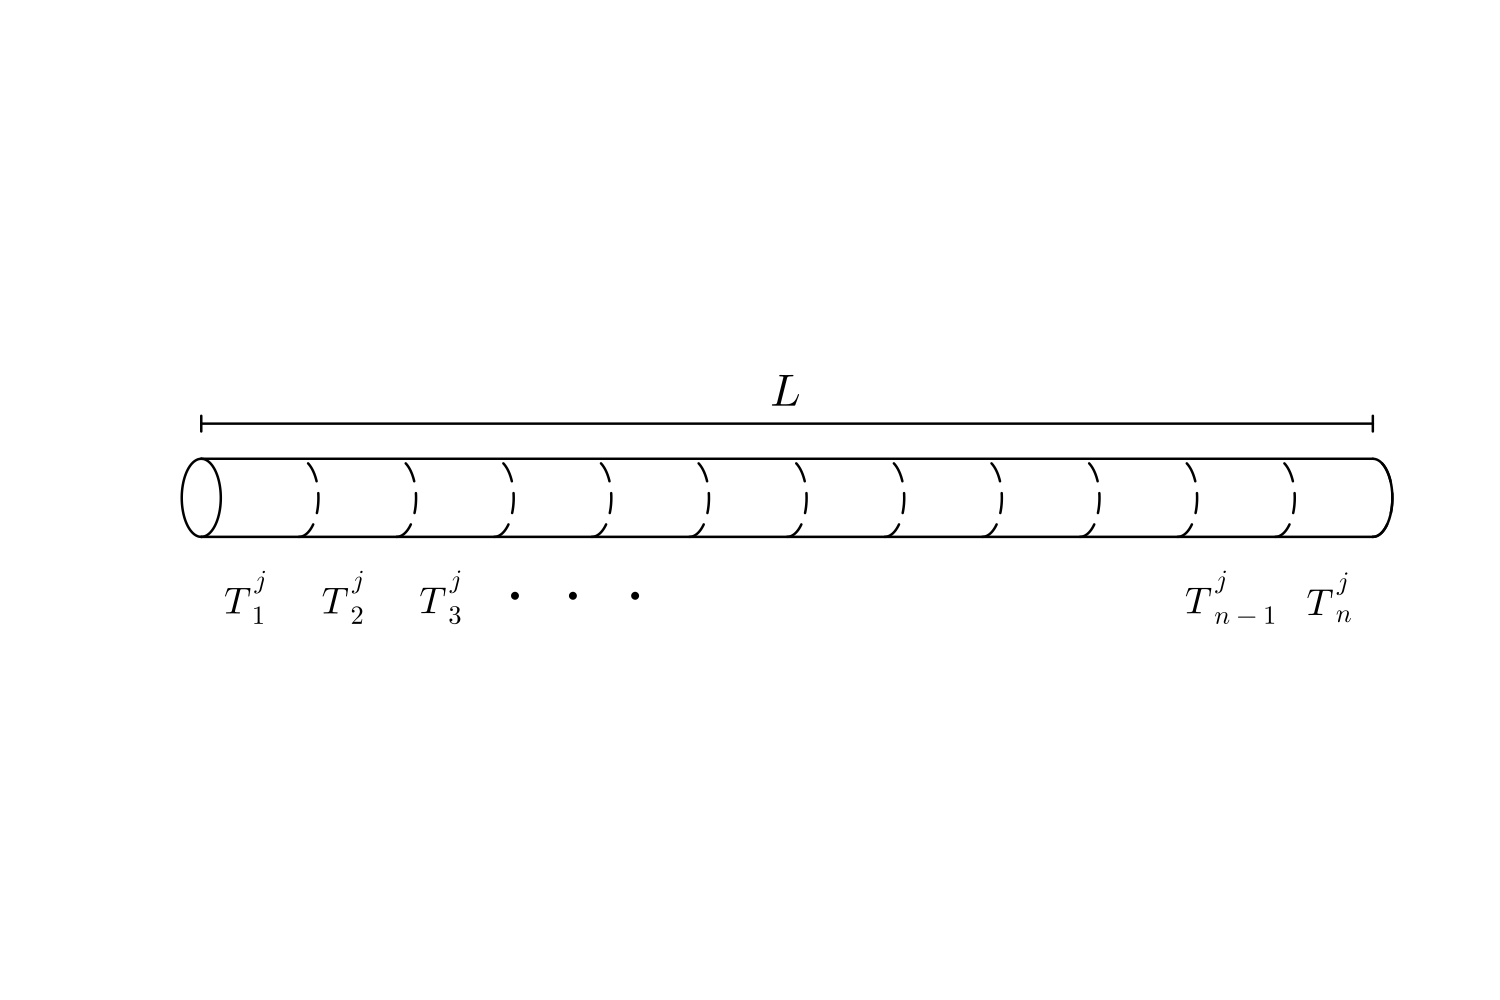
\includegraphics[width=1\linewidth]{Division.png}
    \caption{División de la barra conductora de calor con los elementos $T_i^j$ asociados.}
\end{center}
\end{figure}

De esta manera, si tomamos el i-esimo elemento de la partición realizada a la barra, esta tiene una temperatura que depende del número de paso de tiempo en el que nos encontremos. Si estamos en el j-esimo paso de tiempo, entonces podemos reescribir la notación para la función de temperatura como $T(x,t) = T_i^j$, donde $i$ representa a su posición en el espacio, mientras que $j$ representa su posición en el tiempo, con lo cual podemos escribir la ecuación anterior de la siguiente forma:

\begin{align}
    \kappa T_{i+1}^j + \kappa T_{i-1}^j - [2\kappa + \alpha^2 h]T_i^j = -\alpha^2 h T_i^{j-1}
\end{align}

Esta ecuación es valida para $i \in \{2,3,4,...,n-2,n-1\}$ y para $j \in \{ 2,3,4,... \}$ con lo cual, para un instante en el tiempo, tenemos un sistema de $n-2$ ecuaciones con $n$ incógnitas (los elementos $T_1^j$, $T_2^j$,...,$T_{n-1}^j$,$T_n^j$). Para esto suponemos que conocemos la temperatura de la barra en un paso de tiempo anterior al que estamos calculando (el elemento $T_i^{j-1}$) ya sea por la condición inicial impuesta al sistema o porque este mismo procedimiento se realizó para el paso anterior. \\

Por otro lado, si queremos que el sistema de ecuaciones tenga solución necesitamos dos ecuaciones más, las cuales se obtienen de las condiciones de frontera. Si por ejemplo tenemos condiciones de tipo Dirichlet, las ecuaciones serían:

\begin{align}
    \begin{cases}
        T_1^j = T_1\\
        T_n^j = T_2
    \end{cases}
\end{align}

mientras que, si se tienen condiciones de frontera de tipo Neumann, y considerando las aproximaciones derecha e izquierda de la derivada, llegamos a las siguientes dos ecuaciones:

\begin{align}
    \begin{cases}
        T_2^j - T_1^j = \alpha hC_1\\
        T_n^j - T_{n-1}^j = \alpha hC_2
    \end{cases}
\end{align}

De esta manera, al resolver el sistema de $n-2$ ecuaciones dadas por la expresión (25) junto con dos ecuaciones obtenidas de las condiciones de frontera (ya sea (26) o (27)), podemos obtener todos los valores de $T_i^j$ para todo $i \in \{1,2,3,4,...,n-1,n\}$ lo que se traduce en conocer la temperatura de la barra en cualquier punto de esta para el paso de tiempo $j$. Si ahora queremos saber qué pasa con la barra en el siguiente paso de tiempo, simplemente hay que repetir este procedimiento con la información de la temperatura de la barra obtenida en el paso anterior. Todo este desarrollo nos permite conocer la temperatura de la barra en cualquier punto y en cualquier instante del tiempo al resolver un sistema de ecuaciones lineales. \\

Veamos ahora cómo se compara la solución numérica utilizando el método de diferencias finitas con la solución analítica para la ecuación del calor en una dimensión. Para esto consideraremos una barra con una longitud de $2 \; m$ sujeto a la ecuación de calor en una dimensión, así como las siguientes condiciones:

\begin{align}
    \begin{cases}
        T(x,0) = -x^2 + 2x \;\;\;\;\;\;\;\; \forall x \in [0,2]\\
        T(0,t) = T(2,t) = 0 \;\;\;\;\;\; \forall t>0
    \end{cases}
\end{align}

donde $x$ se mide en metros, $t$ en segundos y la temperatura en Kelvin. Las figuras 4-9 muestran la evolución del sistema en diferentes tiempos considerando condiciones de Dirichlet, es decir, los extremos de la barra siempre tienen una temperatura constante (en este caso $295 \; K$). Además, para este problema se tomó en cuenta un valor de $\kappa = 1.5 \times 10^{-4}$ para la difusividad térmica, valor cercano al del aluminio a temperatura ambiente. \\

\begin{figure}[H]
\begin{center}
    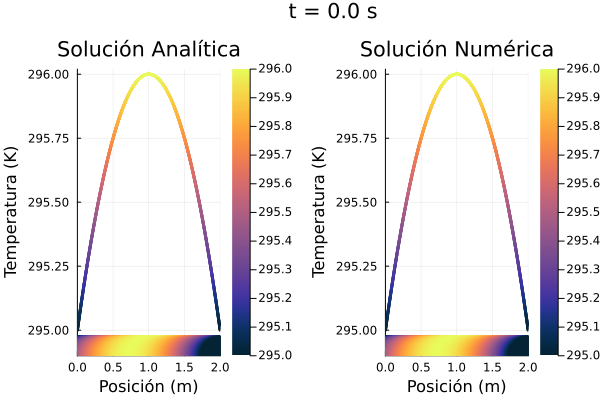
\includegraphics[width=0.79\linewidth]{Ejemplo_01_t_0.png}
    \caption{Comparación entre la solución analítica (izquierda) y la solución numérica (derecha) a la ecuación de calor para las condiciones (28) en el tiempo $t=0 \; s$.}
\end{center}
\end{figure}

\begin{figure}[H]
\begin{center}
    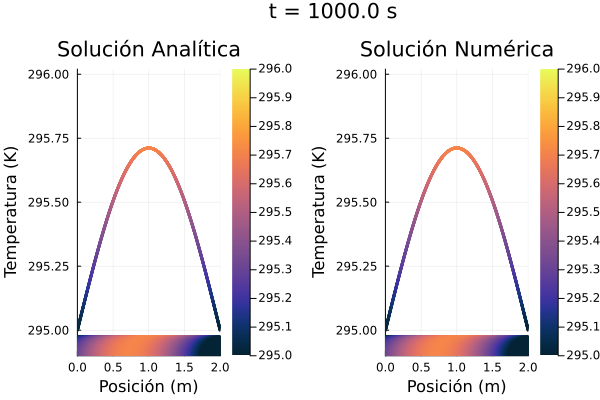
\includegraphics[width=0.79\linewidth]{Ejemplo_01_t_1.png}
    \caption{Comparación entre la solución analítica (izquierda) y la solución numérica (derecha) a la ecuación de calor para las condiciones (28) en el tiempo $t=1000 \; s$.}
\end{center}
\end{figure}

\begin{figure}[H]
\begin{center}
    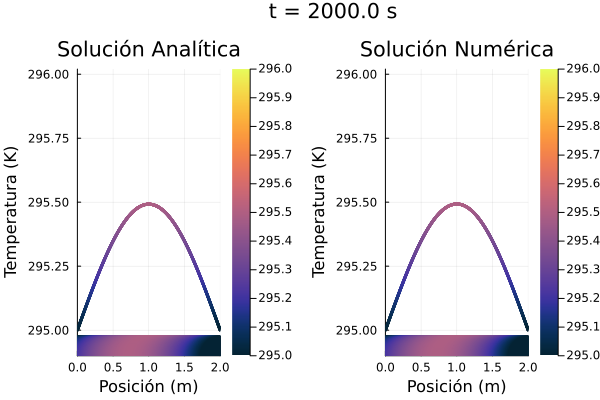
\includegraphics[width=0.79\linewidth]{Ejemplo_01_t_2.png}
    \caption{Comparación entre la solución analítica (izquierda) y la solución numérica (derecha) a la ecuación de calor para las condiciones (28) en el tiempo $t=2000 \; s$.}
\end{center}
\end{figure}

\begin{figure}[H]
\begin{center}
    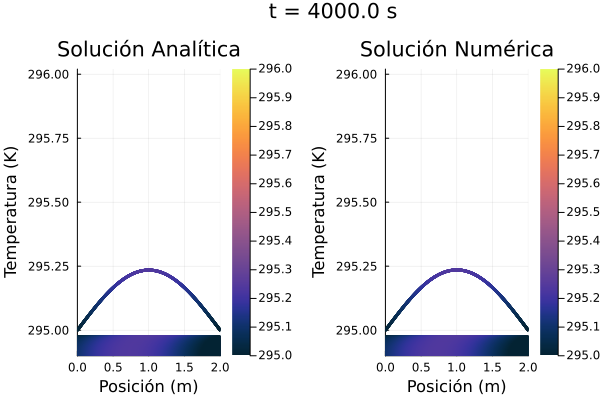
\includegraphics[width=0.79\linewidth]{Ejemplo_01_t_3.png}
    \caption{Comparación entre la solución analítica (izquierda) y la solución numérica (derecha) a la ecuación de calor para las condiciones (28) en el tiempo $t=4000 \; s$.}
\end{center}
\end{figure}

\begin{figure}[H]
\begin{center}
    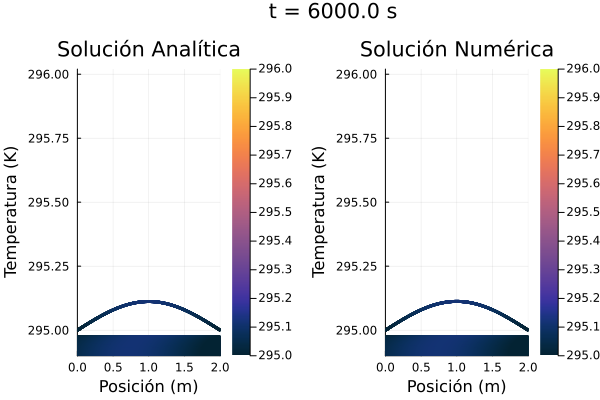
\includegraphics[width=0.79\linewidth]{Ejemplo_01_t_4.png}
    \caption{Comparación entre la solución analítica (izquierda) y la solución numérica (derecha) a la ecuación de calor para las condiciones (28) en el tiempo $t=6000 \; s$.}
\end{center}
\end{figure}

\begin{figure}[H]
\begin{center}
    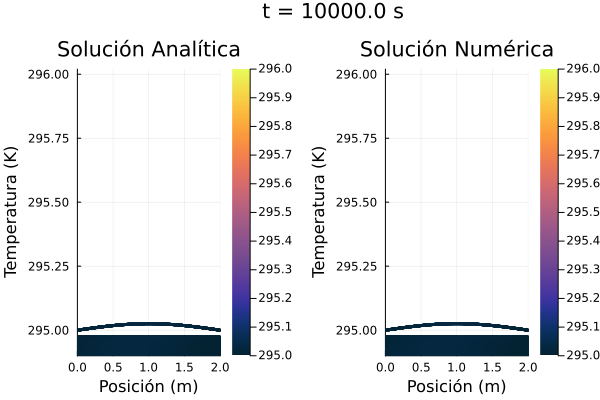
\includegraphics[width=0.79\linewidth]{Ejemplo_01_t_6.png}
    \caption{Comparación entre la solución analítica (izquierda) y la solución numérica (derecha) a la ecuación de calor para las condiciones (28) en el tiempo $t=10000 \; s$.}
\end{center}
\end{figure}

Por otro lado, si consideramos el mismo sistema esta vez con condiciones de frontera de Neumann, lo que significa que los extremos de la barra no permiten el flujo de calor hacia el exterior, tenemos el siguiente conjunto de condiciones:

\begin{align}
    \begin{cases}
        T(x,0) = -x^2 + 2x \;\;\;\;\;\;\;\; \forall x \in [0,2]\\
        \frac{\partial T}{\partial x} \Big|_0 = \frac{\partial T}{\partial x} \Big|_2 = 0 \;\;\;\;\;\;\;\;\;\;\;\;\;\; \forall t>0
    \end{cases}
\end{align}

En las figuras 10-15 se muestra el desarrollo temporal para este problema:


\begin{figure}[H]
\begin{center}
    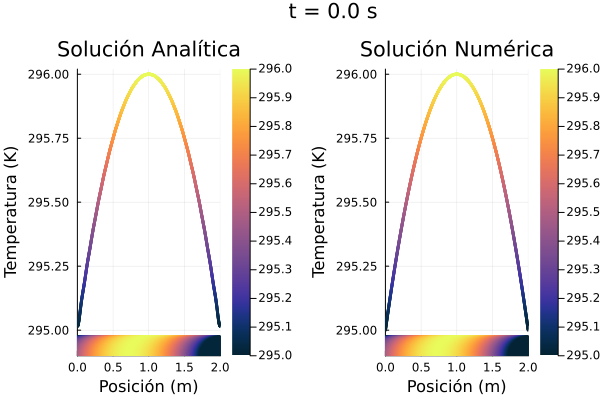
\includegraphics[width=0.79\linewidth]{Ejemplo_02_t_0.png}
    \caption{Comparación entre la solución analítica (izquierda) y la solución numérica (derecha) a la ecuación de calor para las condiciones (29) en el tiempo $t=0 \; s$.}
\end{center}
\end{figure}

\begin{figure}[H]
\begin{center}
    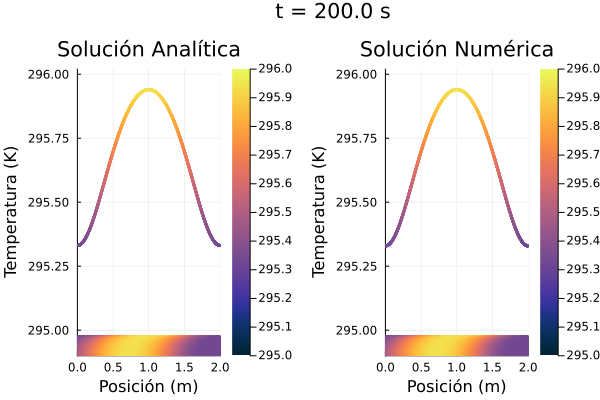
\includegraphics[width=0.79\linewidth]{Ejemplo_02_t_1.png}
    \caption{Comparación entre la solución analítica (izquierda) y la solución numérica (derecha) a la ecuación de calor para las condiciones (29) en el tiempo $t=200 \; s$.}
\end{center}
\end{figure}

\begin{figure}[H]
\begin{center}
    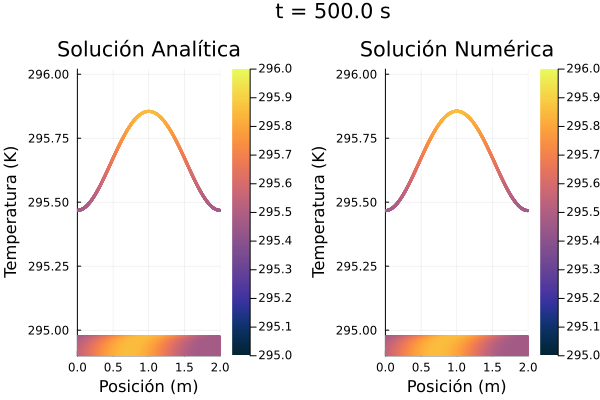
\includegraphics[width=0.79\linewidth]{Ejemplo_02_t_2.png}
    \caption{Comparación entre la solución analítica (izquierda) y la solución numérica (derecha) a la ecuación de calor para las condiciones (29) en el tiempo $t=500 \; s$.}
\end{center}
\end{figure}

\begin{figure}[H]
\begin{center}
    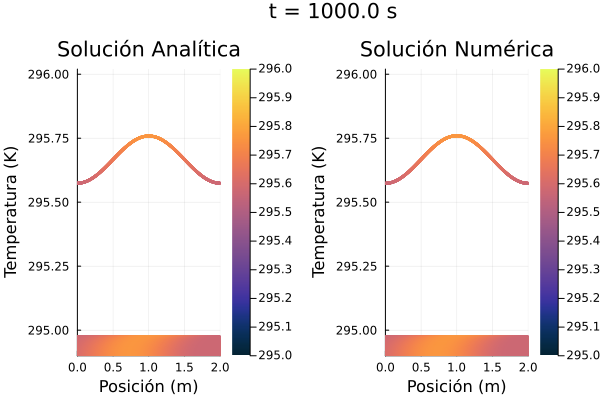
\includegraphics[width=0.79\linewidth]{Ejemplo_02_t_3.png}
    \caption{Comparación entre la solución analítica (izquierda) y la solución numérica (derecha) a la ecuación de calor para las condiciones (29) en el tiempo $t=1000 \; s$.}
\end{center}
\end{figure}

\begin{figure}[H]
\begin{center}
    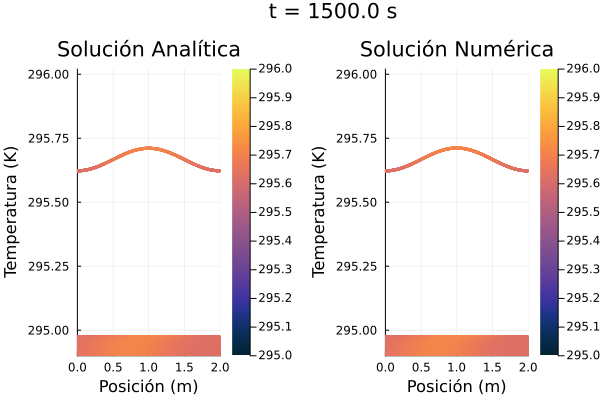
\includegraphics[width=0.79\linewidth]{Ejemplo_02_t_4.png}
    \caption{Comparación entre la solución analítica (izquierda) y la solución numérica (derecha) a la ecuación de calor para las condiciones (29) en el tiempo $t=1500 \; s$.}
\end{center}
\end{figure}

\begin{figure}[H]
\begin{center}
    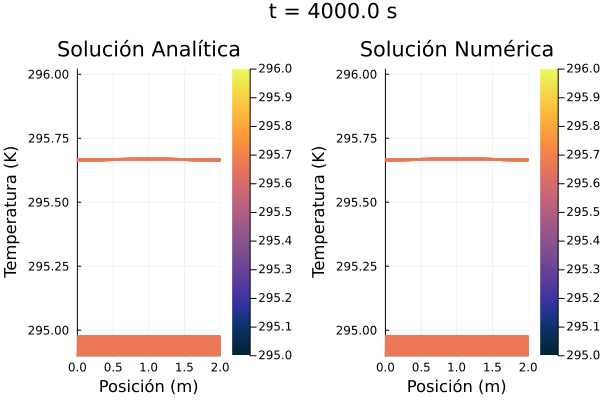
\includegraphics[width=0.79\linewidth]{Ejemplo_02_t_6.png}
    \caption{Comparación entre la solución analítica (izquierda) y la solución numérica (derecha) a la ecuación de calor para las condiciones (29) en el tiempo $t=4000 \; s$.}
\end{center}
\end{figure}

Si ahora queremos aplicar este método a dos dimensiones, se repite el mismo procedimiento, considerando una cantidad de elementos $T_i^j$ mayor. Para ejemplificar esto, tomemos una placa rectangular cuyos lados miden $L_1$ y $L_2$ y la dividiremos en $m$ columnas y $n$ renglones. Para simplificar este problema supondremos que cada división es del mismo tamaño (tanto de renglones como de columnas) de esta manera, cada división mide $h_x = L_1/n = L_2/m$. \\

La numeración de los elementos de temperatura se hace de izquierda a derecha y de arriba hacia abajo de tal manera que, para un elemento de tiempo dado $j$, las divisiones del primer renglón tienen temperaturas de $T_1^j$, $T_2^j$, ..., $T_m^j$ para el segundo renglón se tienen temperaturas $T_{m+1}^j$, $T_{m+2}^j$, ..., $T_{2m}^j$ y así sucesivamente hasta llegar al último renglón que tiene temperaturas $T_{m(n-1)+1}^j$, $T_{m(n-1)+2}^j$, ..., $T_{nm}^j$.

\begin{figure}[H]
\begin{center}
    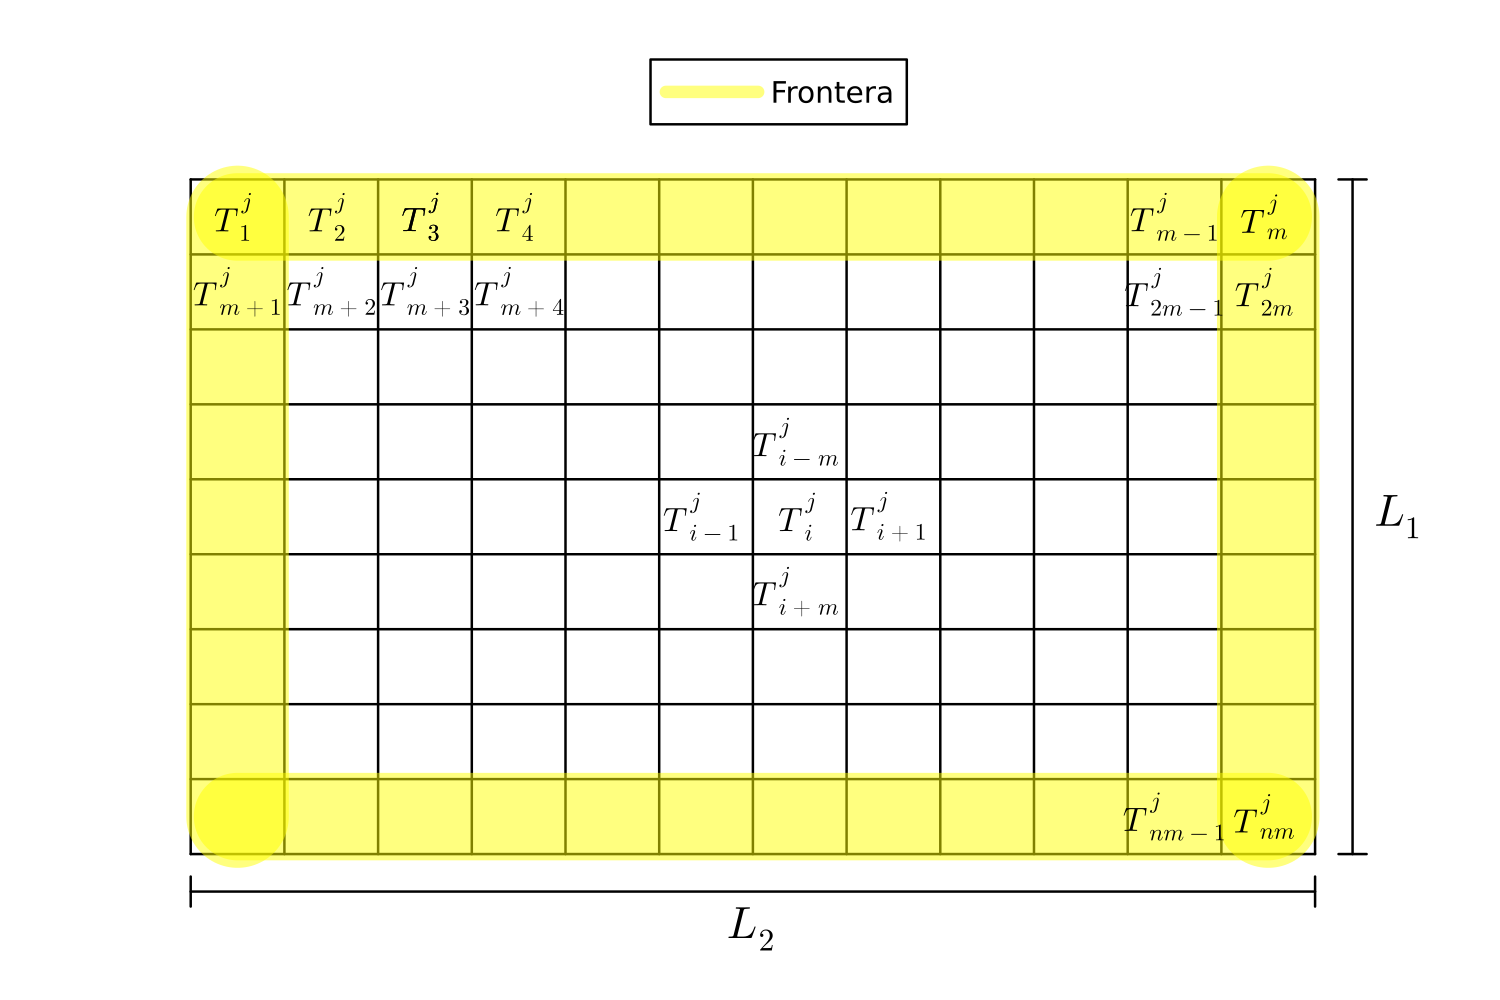
\includegraphics[width=1\linewidth]{Placa.png}
    \caption{Diagrama de una placa de dimensiones $L_1$ y $L_2$ con los elementos de temperatura $T_i^j$ en cada división.}
\end{center}
\end{figure}

La ecuación del calor para este sistema es ahora:

\begin{align*}
    \frac{\partial T}{\partial t} = \kappa \frac{\partial^2 T}{\partial x^2} + \kappa \frac{\partial^2 T}{\partial y^2}
\end{align*}

Tomando las mismas aproximaciones para la derivada que en el caso de una dimensión:

\begin{align*}
    \frac{T(x,y,t)-T(x,y,t-h_t)}{h_t} = &\kappa \frac{T(x+h_x,y,t) - 2T(x,y,t) + T(x-h_x,y,t)}{h_x^2} \\
    +&\kappa \frac{T(x,y+h_x,t) - 2T(x,y,t) + T(x,y-h_x,t)}{h_x^2}
\end{align*}

reordenando los términos con los elementos $T_i^j$ llegamos a la expresión:

\begin{align}
    \kappa T_{i+1}^j + \kappa T_{i-1}^j + \kappa T_{i-m} + \kappa T_{i+m} - [4\kappa + \alpha^2 h]T_i^j = -\alpha^2 h T_i^{j-1}
\end{align}

La ecuación (30) es valida para cualquier elemento $T_i^j$ que no pertenezca a la frontera de la placa y, al igual que en el caso de una dimensión, para que se tenga un sistema de ecuaciones con solución es necesario obtener el resto de ecuaciones de las condiciones de frontera. Podemos notar ademas que la temperatura en una de las divisiones de la placa depende de sus vecinos, que esta vez son los elementos $T_{i+1}^j$, $T_{i-1}^j$, $T_{i+m}^j$ y $T_{i-m}^j$. Así, al resolver este sistema de ecuaciones, podemos obtener la temperatura para cada división en un instante de tiempo dado $j$.

\subsection{Objetivos}
\subsection{Hipótesis}

\section{Desarrollo experimental}

\newpage

\subsection{Dispositivo de medición}

Como ya se mencionó en la sección anterior, al resolver la ecuación de calor obtendremos una función que, a cada instante del tiempo, nos dará la temperatura de cada punto en el espacio. Con el fin de comparar los resultados obtenidos a través de una simulación computacional, es necesario llevar a cabo un experimento en el cual se mida la temperatura en una región del espacio durante un determinado intervalo de tiempo. Para ello es indispensable un dispositivo capaz de medir la temperatura en una serie de puntos, así como de almacenar y mostrar gráficamente los datos obtenidos. En las siguientes secciones se realiza una descripción de los elementos utilizados en la construcción de dicho dispositivo.


\subsubsection{Arduino}

En primer lugar, es necesario un procesador capaz de recibir y enviar diversas señales analógicas y digitales con el fin de controlar el dispositivo, para lo cual se eligió una tarjeta de desarrollo Arduino Mega 2560. \\

Arduino es una plataforma de desarrollo que incorpora Hardware y Software libre, la cual es ampliamente utilizada en diversos proyectos de electrónica por su capacidad de controlar dispositivos y/o circuitos al recibir y emitir señales tanto analógicas como digitales de forma práctica y sencilla. El hardware se compone de diferentes placas de desarrollo, cada una empleada en distintos contextos dependiendo de sus características. Para poder dar instrucciones a estas placas se utiliza el lenguaje de programación de Arduino basado en C, así como un Entorno de Desarrollo Integrado llamado Arduino IDE, el cual cuenta con un editor de texto, un compilador, y muchas otras herramientas que facilitan el desarrollo de código. \\

La placa Mega 2560 está basada en el microprocesador AT-mega 2560, cuenta con 54 pines digitales, de los cuales 14 son PWM, 16 pines analógicos, una memoria Flash de $256 \; kB$, SRAM de $8 \; kB$ y una EEPROM de $4 \; kB$. Su voltaje de operación es de $5 \; V$ con una corriente en cada pin de $20 \; mA$ y sus dimensiones son: $10.2 \; cm \; \times \; 1.8 \; cm$. La elección de esta placa por encima del resto de tarjetas de desarrollo que ofrece Arduino se debe a su gran cantidad de pines, característica necesaria para que el dispositivo a construir tenga la capacidad de recibir datos de un número considerable de sensores. Además de esto, la placa Mega 2560 cuenta con una de las memorias más grandes dentro de las tarjetas de desarrollo de Arduino, lo que permite crear un código para controlar la placa tan grande como sea necesario sin comprometer el buen funcionamiento de la misma. \\

El código que permite el funcionamiento de la placa se escribe en un archivo con extensión .ino, el cual es creado en el programa Arduino IDE y es guardado en un directorio con el mismo nombre del archivo. Este código se compone principalmente de dos funciones: la primera de ellas se llama \textbf{setup} y sirve para inicializar y configurar los sensores y demás elementos electrónicos que se conectaran a la tarjeta de desarrollo. También permite declarar variables, inicializar y configurar un protocolo de comunicación entre la placa y algún otro dispositivo como un ordenador, etc. Esta función es la primera que se ejecuta dentro de la placa y lo hará en una solo ocasión (a menos que desde el código se llame a la función \textbf{setup} en otra linea). \\

La segunda función principal del código es \textbf{loop} y en ella se pondrán todas aquellas instrucciones que se quieran repetir constantemente, pues dicha función se ejecuta de forma cíclica después de que es ejecutada la función \textbf{setup}. Aquí es común leer los valores de los dispositivos de entrada como sensores y dar instrucciones en función de dichos valores a los dispositivos de salida como motores, lectores de memoria, etc. \\

Fuera de las dos funciones principales mencionadas anteriormente, es posible crear más funciones que sean llamadas ya sea en \textbf{setup} o en \textbf{loop}, así como declarar variables globales, llamar a librerías que estén instaladas en el entorno de desarrollo, entre otras acciones e instrucciones. Finalmente, para cargar el programa es necesario conectar un cable USB tipo B hembra desde el ordenador donde se escribió el código hasta la placa de desarrollo y dar click en la opción de cargar programa, la cual se puede encontrar en el programa Arduino IDE. \\


\subsubsection{Sensor ds18b20}

Después de escoger un microprocesador capaz de controlar el dispositivo de medición, es necesario seleccionar el sensor que se encargará de medir la magnitud física de nuestro interés, en este caso la temperatura. Para ello se seleccionó el termómetro digital \textbf{ds18b20} capaz de proporcionar medidas de temperatura en Celsius con una resolución de 9 a 12 bits configurable, un rango que va de los $-55 \; ^{\circ}C$ hasta los $125 \; ^{\circ}C$ y una presición de $\pm 0.5 ^{\circ}C$ en el intervalo de temperaturas de $-10 \; ^{\circ}C$ a $85 \; ^{\circ}C$. \\



\subsubsection{Protocolo de comunicación OneWire}


\subsection{Circuito y montaje lineal (10 sensores)}
\subsection{Circuito y montaje en una placa (200 sensores)}
\subsection{Toma y tratamiento de datos}
\subsection{Simulación computacional}

\section{Resultados}
\subsection{Mediciones lineales}
\subsection{Mediciones en la placa}
\subsection{Resultados de la simulación}
\subsection{Conclusiones}



\end{document}
